\chapter{Wstęp}
\thispagestyle{chapterBeginStyle}
\label{rozdzial1}

W \textit{Teori Grafów} kolorowanie grafu jest szczególnym przypadkiem etykietowania, tradycyjnie nazywanymi kolorami. 
\textit{Minimalne Kolorowanie Grafu} etykietuje wierzchołki (kolorami) tak bym, żadna krawędź nie łączyła dwóch wierzchołków o tej samej etykiecie (kolorze).
Minimalna ilość kolorów potrzebna do \textit{Minimalnego Kolorowania Grafu} nazywana jest \textit{Liczbą Chromantyczną} samo wyznaczenie tej liczby jest problemem \textit{NP-trudnym}\cite{NP}, dlatego nie ma wielomianowego algorytmu rozwiązującego zadanie. 

Zastosowaniem algorytmu rozwiązującego kolorowanie grafu, może być szeregowanie zadań. 
Gdzie wierzchołki są zadaniami, a krawędzie pomiędzy nimi zasobem współdzielonym.
Rozwiązanie problemu mówiło by w jaki sposób uruchamiać grupy zadań,
by zasób wspódzielony wykorzystywany byłby przez jedną maszynę na raz.

Problemem z życia może być układanie planu zajęć, gdzie krawędziami są sale lub lektorzy, a wierzchołkami ilość zajęć.  
Liczba kolorów mówiłaby ile godzin zajęciowych potrzebnych jest do zrealizowania planu, a grupy wierzchołków prezentowały by jakie zajęcia mogą obywać się o jednej godzinie.


\section{Opis problemu}
\textit{Minimalne Kolorowanie Grafu} jest przypisaniem kolorów do każdego wierzchołka grafu, tak że żadna krawędź nie łączy dwóch identycznie pokolorowanych wierzchołków.
Problemem jest znalezienie takiego etykietowania by nie można było znaleźć etykietowania z mniejszą ilością kolorów.

\subsection{Model}
\begin{itemize}
    \item Dane: Graf $G(V, E)$ gdzie $V$ to wierzchołki, a $E$ to krawędzie. 
    \item Rozwiązanie: Kolorowanie $G$, tj. podział wierzchołków $V$ na zbiory $V_1, V_2, ..., V_k$  , takie że każdy zbiór $V_i$ jest niezależny w $G$.
    \item Miara: Ilość zbiorów $V_i$
\end{itemize}

\clearpage


\section{Przykłady}
Poniżej zostały przedstawione przykłady rozwiązania problemu \textit{Minimalnego Kolorowania Grafu} z
 różnymi rodzajami grafów. Omawiane grafy przedstawione są na rysunkach \ref{Przyklady}.

 \begin{itemize}
    \item \textit{Graf pełny} rozwiązaniem dla niego jest $|V|$, ponieważ każdy wierzchołek posiada krawędź z
     pozostałymi wierzchołkami, dlatego każdy z nich musi mieć inny kolor.
    \item \textit{Graf k-dzielny} jego definicja opisuje szukane rozwiązanie dla \textit{Minimalnego Kolorowania Grafu}, tzn. wartość $k$  \textit{k-dzielności grafu} opisuje rozwiązanie. W rysunku \textit{b} został przedstawiony graf \textit{graf 3-dzielny}, gdzie kolory wierzchołków opisują grupy do której należą.
    \item \textit{Graf planarny} każdy graf prosty tego rodzaju jest co najwyżej $4-kolorowalny$ \cite{4colorable}. Na przedstawionym przykładzie grafu planarnego widać, że nie można znaleźć miejsca dla wierzchołka połączonego z czteroma wierzchołkami o różnych kolorach, nie przecinając istniejącej krawędzi.
    \item Dla pozostałych grafów przedstawione zostało górne ograniczenie \textit{Kolorowanie grafu}, znane jako \textit{Twierdzenie Brooksa} \cite{brooks_1941}. 
    Ustala że \textit{liczba chromatyczna} jest niewiększa niż maksymalny stopień wierzchołka ($max(deg(V))$), z wyjątkiem
     \textit{grafu z nieparzystym cyklem} wtedy wartość jest nie większa niż $max(deg(V)) + 1$.
\end{itemize}


\begin{figure}
    \begin{subfigure}[t]{0.4\textwidth}
      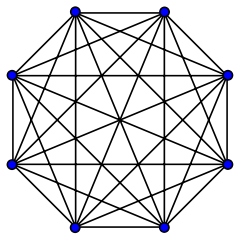
\includegraphics[width=\textwidth]{grafpelny.png}
      \caption{Graf Pełny o 8 wierzchołkach - rozwiązaniem jest 8}
    \end{subfigure}
    \hfill
    \begin{subfigure}[t]{0.4\textwidth}
      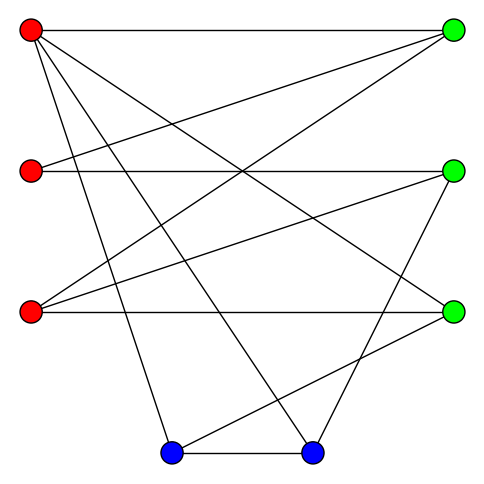
\includegraphics[width=\textwidth]{3dzielny.png}
      \caption{Graf 3-dzielny - rozwiązaniem jego jest 3}
    \end{subfigure}
    \begin{subfigure}[t]{0.3\textwidth}
        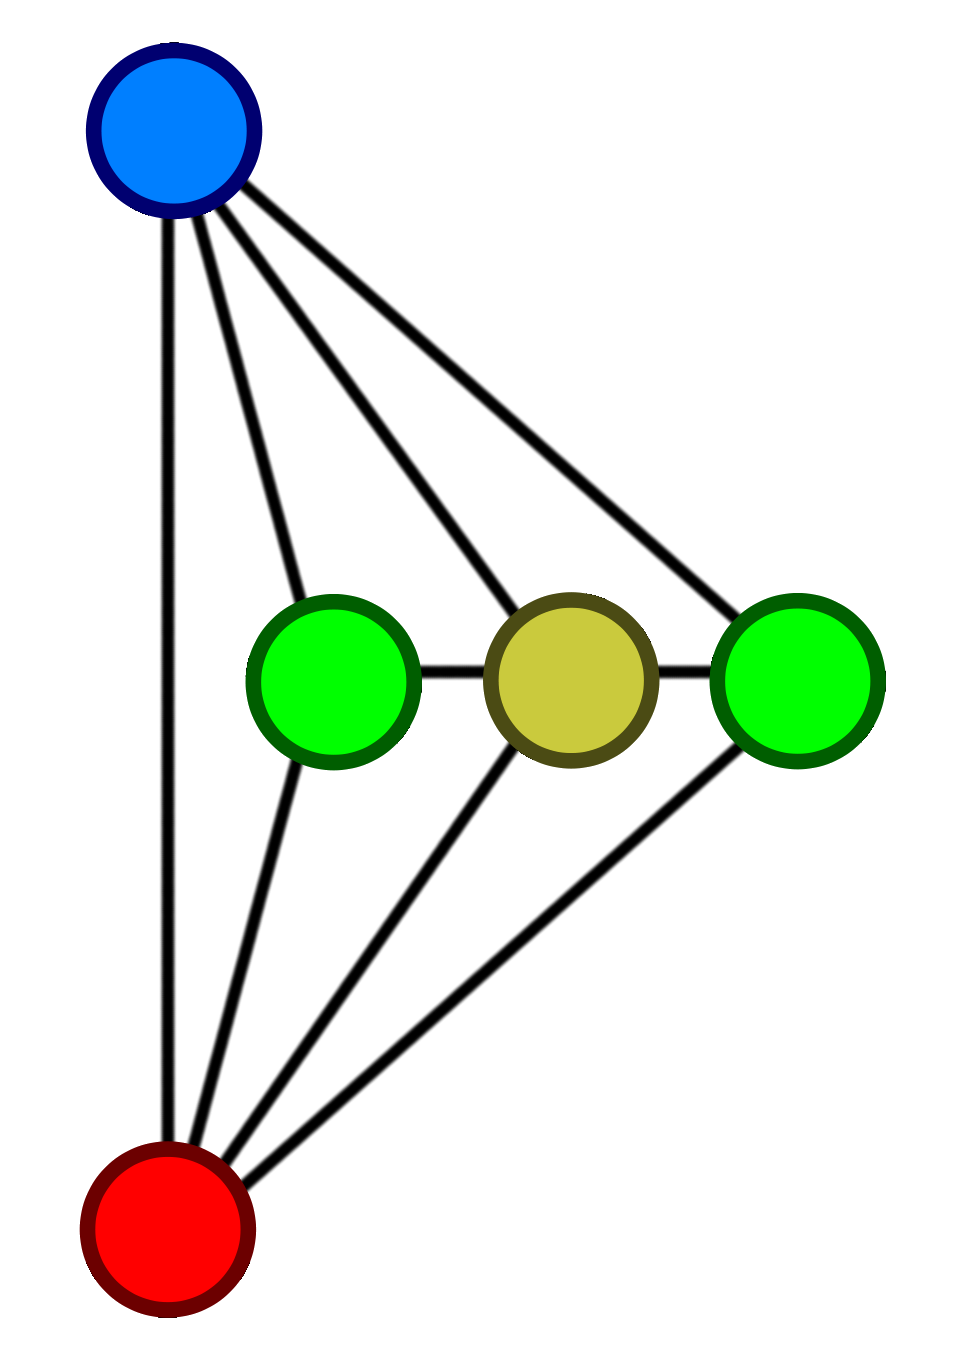
\includegraphics[width=\textwidth]{planarny.png}
        \caption{Graf planarny - rozwiązaniem jego jest 4}
    \end{subfigure}
    \hfill
    \begin{subfigure}[t]{0.3\textwidth}
        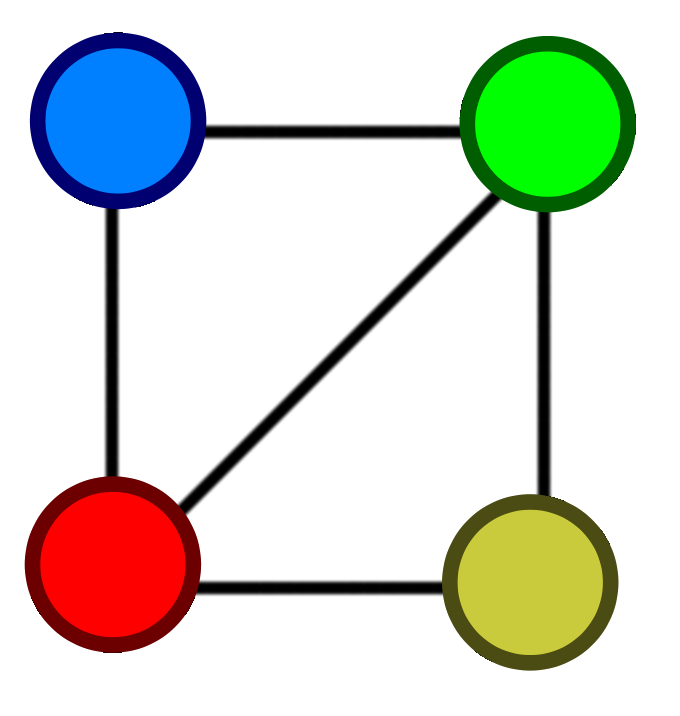
\includegraphics[width=\textwidth]{cycle.png}
        \caption{Graf z cyklem nieparzystym - maksymalny stopień 3, rozwiązaniem jego jest 4}
    \end{subfigure}
    \hfill
    \begin{subfigure}[t]{0.3\textwidth}
        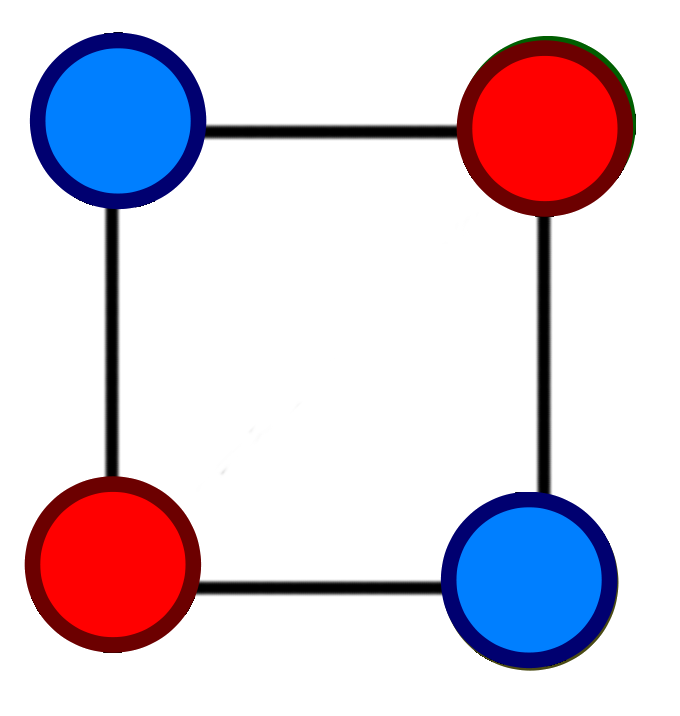
\includegraphics[width=\textwidth]{ncycle.png}
        \caption{Graf bez cyklu nieparzystego - maksymalny stopień 2, rozwiązaniem jego jest 2}
    \end{subfigure}
    \caption{Przykładowe grafy}
    \label{Przyklady}
\end{figure}




\iffalse

\begin{table}[ht]
    \begin{center}
        \begin{tabular}{|c | c| c| c| c|} 
            \hline
            \rowcolor{lgray}
            ilość & 7cal & 5cal & 3cal & odpad \\
            \hline
            9 & 1 & 0 & 5 & 0\\
            \hline
            28 & 1 & 3 & 0 & 0\\
            \hline
            37 & 2 & 1 & 1 & 0\\
            \hline
            \rowcolor{lgray}
            suma & 111 & 121 & 82 & 0\\
            \hline
        \end{tabular}
        \caption{Podział desek}
        \label{tabela_zad1}
    \end{center}
\end{table}

Rozwiązanie przykładu podanego w zadaniu \ref{zadanie3}. Rozwiązanie zostało zaprezentowane w tabeli \ref{tabela_zad3}
\begin{figure}[h]
    \centering
    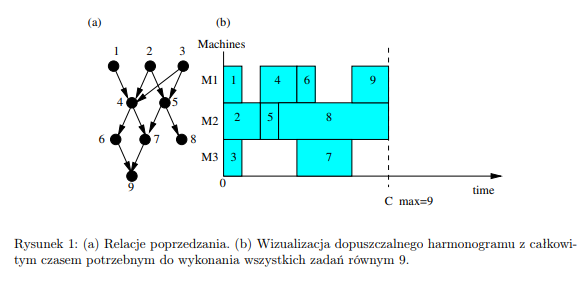
\includegraphics[scale=1.0]{zadanie3.png}
    \caption{Dane i rozwiązanie}
    \label{zadanie3}
\end{figure}


\fi